\chapter{[matplotlib] 绘图}
\section{折线/散点图}
\subsection{plt.plot 折线/散点图}
\codeinline{plt.plot()} 用于绘制散点图，默认情况下，\codeinline{plt.plot(x, y)} 会连接每个点，生成一条平滑的连线图。

\begin{lstlisting}[style=demostyle,numbers=none]
# 必须导入的库
import matplotlib.pyplot as plt
# plot 功能：用于绘制散点图
plt.plot(*args, scalex=True, scaley=True, data=None, **kwargs)
# 参数说明：
# x : x坐标
# y : y坐标
# fmt : 线条样式
## 'o'：点
## '-o'：点连线
## '-H'：六边形连线
# data : 数据源
# scalex, scaley : 是否自动缩放x或y轴
\end{lstlisting}

\begin{lstlisting}[style=pythonstyle]
import numpy as np
import matplotlib.pyplot as plt

# 生成从 0 到 1.1，步长为 0.01 的数据
data = np.arange(0, 1.1, 0.01)

# 设置图表的标题
plt.title('lines')  # 添加标题

# 设置 x 轴和 y 轴的名称
plt.xlabel('x')  # 添加 x 轴的名称
plt.ylabel('y')  # 添加 y 轴的名称

# 设置 x 轴和 y 轴的范围
plt.xlim((0, 1))  # 确定 x 轴范围
plt.ylim((0, 1))  # 确定 y 轴范围

# 设置 x 轴和 y 轴的刻度
plt.xticks([0, 0.2, 0.4, 0.6, 0.8, 1])  # 规定 x 轴刻度
plt.yticks([0, 0.2, 0.4, 0.6, 0.8, 1])  # 确定 y 轴刻度

# 使用 plot 函数绘制连线图
plt.plot(data, data)  # 绘制 y = x 曲线
plt.plot(data, data**2)  # 绘制 y = x^2 曲线

# 添加图例
plt.legend(['y=x', r'$y=x^2$'])  # r'' 使得数学公式正确显示

# 保存图像
plt.savefig('../tmp/默认连线图.png')

# 显示图像
plt.show()
\end{lstlisting}
\begin{figure}[htpb]
    \centering
    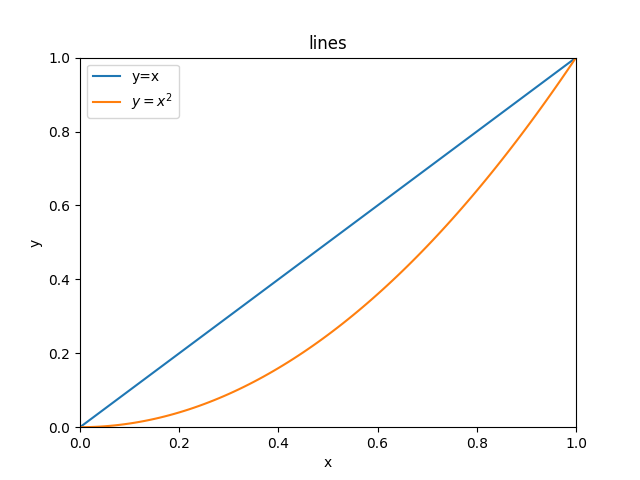
\includegraphics[width=0.4\textwidth]{part/图形化/Matplotlib/pic/绘图/plot默认连线图.png}
    \caption{plot默认连线图}
\end{figure}


\begin{lstlisting}[style=pythonstyle]
import matplotlib.pyplot as plt
import numpy as np
fig = plt.figure(figsize=(6,4))
x = np.linspace(0, 10, 30)
y = np.sin(x)

# 等价于 plt.plot(x, y, mark='o', color='blue')
plt.plot(x, y, 'ob')
\end{lstlisting}
\begin{figure}[htpb]
    \centering
    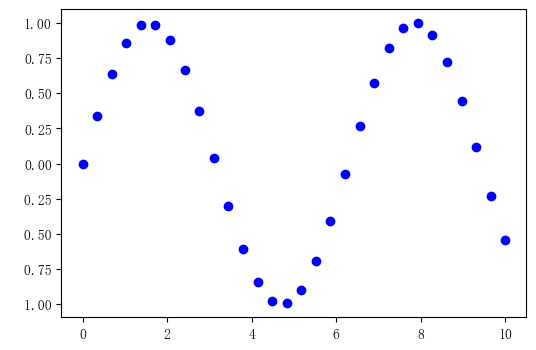
\includegraphics[width=0.6\textwidth]{part/图形化/Matplotlib/pic/绘图/plot散点图.png}
    \caption{plot散点图}
\end{figure}

\begin{lstlisting}[style=demostyle,numbers=none]
$> cat people.csv    
指标,年末总人口(万人),0-14岁人口(万人),15-64岁人口(万人),65岁及以上人口(万人)
2000年,126743,29012,88910,8821
2001年,127627,28716,89849,9062
2002年,128453,28774,90302,9377
2003年,129227,28559,90976,9692
2004年,129988,27947,92184,9857
2005年,130756,26504,94197,10055
2006年,131448,25961,95068,10419
2007年,132129,25660,95833,10636
2008年,132802,25166,96680,10956
2009年,133450,24659,97484,11307
2010年,134091,22259,99938,11894
2011年,134735,22164,100283,12288
2012年,135404,22287,100403,12714
2013年,136072,22329,100582,13161
2014年,136782,22558,100469,13755
2015年,137462,22715,100361,14386
2016年,138271,23008,100260,15003
2017年,139008,23348,99829,15831
2018年,139538,23523,99357,16658
2019年,140005,23493,98914,17599
\end{lstlisting}
\begin{lstlisting}[style=pythonstyle]
import numpy as np
import pandas as pd
import matplotlib.pyplot as plt
plt.rcParams['font.sans-serif'] =' SimHei'
# 设置中文显示
plt.rcParams['axes.unicode_minus'] = False
data = pd.read_csv('../data/people.csv')
name = data.columns  # 提取其中的columns字段，视为数据的标签
values = data.values  # 提取其中的values字段，数据的存在位置
plt.figure(figsize=(9, 7))  # 设置画布
plt.scatter(values[:, 0], values[:, 1], marker='o')  # 绘制散点图
plt.xlabel('年份')  # 添加横轴标签
plt.ylabel('年末总人口（万人）')  # 添加y轴名称
plt.xticks(range(0, 20), values[range(0, 20), 0], rotation=45)
plt.title('2000-2019年年末总人口散点图')  # 添加图表标题
plt.savefig('../tmp/2000-2019年年末总人口散点图.png') # 保存图表
plt.show()
\end{lstlisting}
\begin{figure}[htpb]
    \centering
    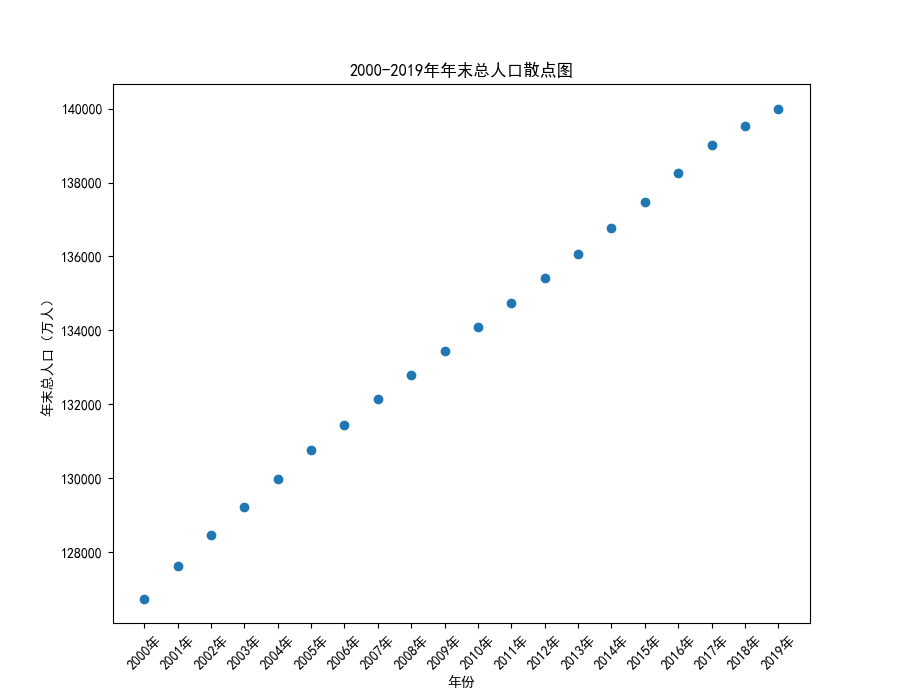
\includegraphics[width=0.6\textwidth]{part/图形化/Matplotlib/pic/绘图/2000-2019年年末总人口散点图.png}
    \caption{2000-2019年年末总人口散点图}
\end{figure}


\subsubsection{-o 将散点图连线}
使用 \codeinline{plt.plot()} 可以绘制连线的散点图。
\begin{lstlisting}[style=pythonstyle]
import matplotlib.pyplot as plt
import numpy as np

# 数据
x = np.linspace(0, 10, 30)
y = np.sin(x)

# 绘制连线的散点图
plt.plot(x, y, '-o', color='blue')  # 使用线条连接散点
plt.title('连线的散点图')
plt.show()
\end{lstlisting}

\begin{figure}[htpb]
    \centering
    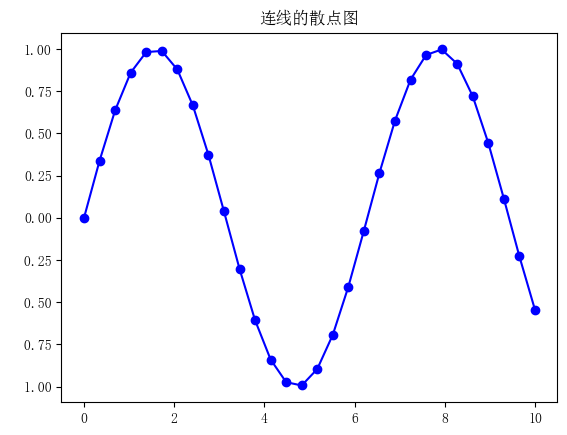
\includegraphics[width=0.6\textwidth]{part/图形化/Matplotlib/pic/绘图/连线的散点图.png}
    \caption{连线的散点图}
\end{figure}

\begin{lstlisting}[style=pythonstyle]
import numpy as np
import pandas as pd
import matplotlib.pyplot as plt

# 设置中文显示
plt.rcParams['font.sans-serif'] = 'SimHei'  # 解决中文乱码问题
plt.rcParams['axes.unicode_minus'] = False  # 设置正常显示负号

# 读取数据
data = pd.read_csv('../data/people.csv')
name = data.columns  # 提取columns字段，视为数据的标签
values = data.values  # 提取values字段，数据的存在位置

# 创建画布，并设置左右两个子图
plt.figure(figsize=(16, 7))  # 设置画布大小

# 左侧子图
plt.subplot(1, 2, 1)  # 创建第一个子图
plt.plot(values[:, 0], values[:, 1], color='r', linestyle='--', marker='o')  # 绘制折线图
plt.xlabel('年份')  # 添加横轴标签
plt.ylabel('年末总人口（万人）')  # 添加y轴名称
plt.xticks(range(0, 20), values[range(0, 20), 0], rotation=45)
plt.title('2000-2019年年末总人口点线图')  # 添加图表标题

# 右侧子图
plt.subplot(1, 2, 2)  # 创建第二个子图
plt.plot(values[:, 0], values[:, 2], 'bs-',  # 蓝色方块实线
         values[:, 0], values[:, 3], 'ro-.',  # 红色圆点虚线
         values[:, 0], values[:, 4], 'gH--')  # 绿色六边形点划线
plt.xlabel('年份')  # 添加横轴标签
plt.ylabel('年末总人口（万人）')  # 添加y轴名称
plt.xticks(range(0, 20), values[range(0, 20), 0], rotation=45)
plt.title('2000-2019年各年龄段总人口点线图')  # 添加图表标题
plt.legend(['0-14岁人口', '15-64岁人口', '65岁及以上人口'])

# 保存合并的图表
plt.tight_layout()  # 调整子图布局，避免重叠
plt.savefig('../tmp/2000-2019年总人口点线图.png')
plt.show()
\end{lstlisting}
\begin{figure}[htpb]
    \centering
    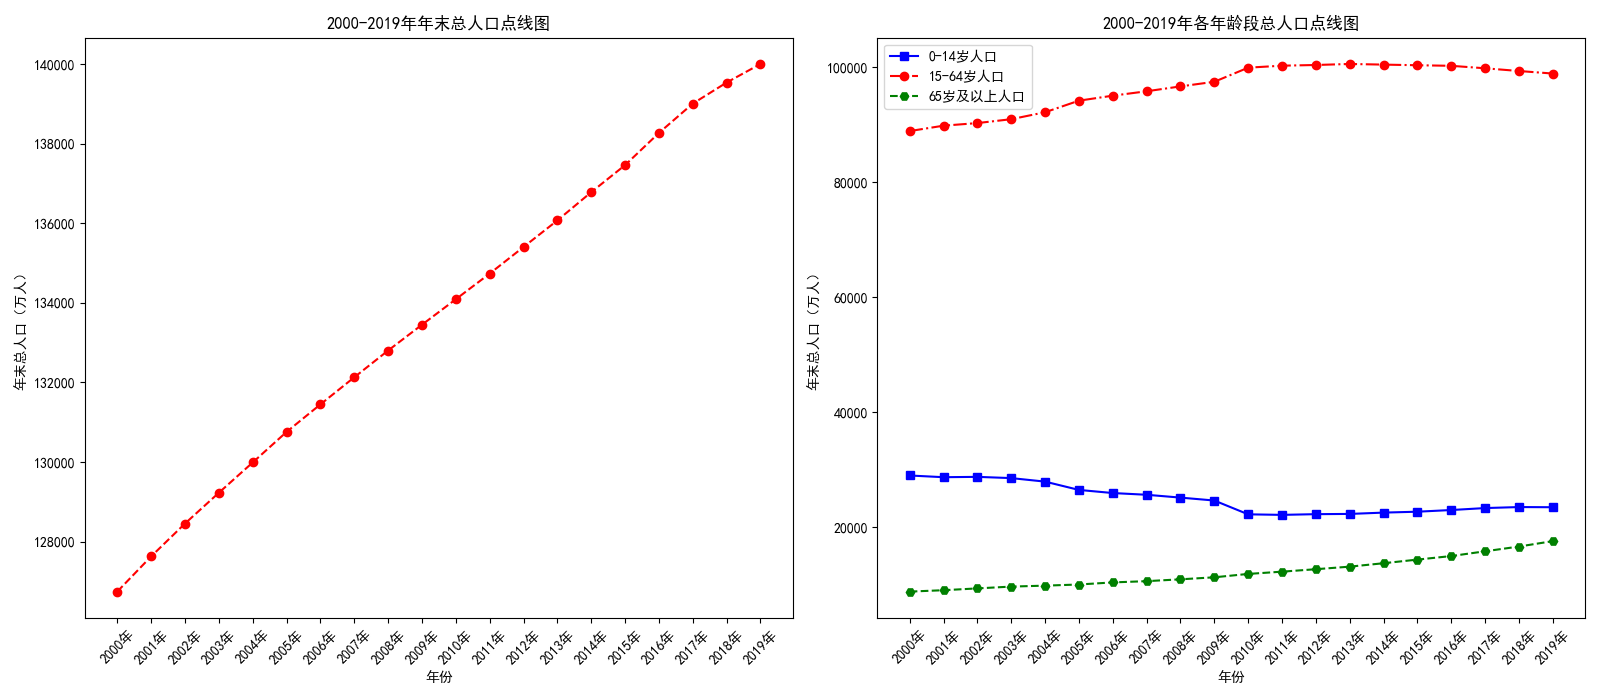
\includegraphics[width=0.6\textwidth]{part/图形化/Matplotlib/pic/绘图/2000-2019年总人口点线图.png}
    \caption{2000-2019年总人口点线图}
\end{figure}



\subsubsection{设置散点图属性}
\begin{lstlisting}[style=pythonstyle]
import matplotlib.pyplot as plt
import numpy as np
fig = plt.figure(figsize=(6,4))
x = np.linspace(0, 10, 30)
y = np.sin(x)

plt.plot(x, y, '-H', color='gray',   # 线条颜色 -H 代表六边形
         markersize=15, linewidth=4, # 标记大小，线宽
         markerfacecolor='white',    # 标记填充色
         markeredgecolor='gray',     # 标记边框色
         markeredgewidth=2)          # 标记边框宽度
\end{lstlisting}

\begin{figure}[htpb]
    \centering
    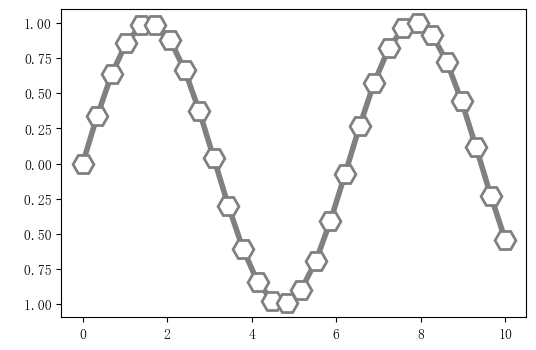
\includegraphics[width=0.6\textwidth]{part/图形化/Matplotlib/pic/绘图/设置散点图属性.png}
    \caption{设置散点图属性}
\end{figure}

\subsubsection{绘制折线图}
\begin{lstlisting}[style=pythonstyle]
import numpy as np
import pandas as pd
import matplotlib.pyplot as plt
plt.rcParams['font.sans-serif'] =' SimHei'
# 设置中文显示
plt.rcParams['axes.unicode_minus'] = False
data = pd.read_csv('../data/people.csv')
name = data.columns  # 提取其中的columns字段，视为数据的标签
values = data.values  # 提取其中的values字段，数据的存在位置    
plt.figure(figsize=(9, 7))  # 设置画布
plt.plot(values[:, 0], values[:, 1], color='r', linestyle='--')  # 绘制折线图
plt.xlabel('年份')  #添加横轴标签
plt.ylabel('年末总人口（万人）')  # 添加y轴名称
plt.xticks(range(0, 20), values[range(0, 20), 0], rotation=45)
plt.title('2000-2019年年末总人口折线图')  # 添加图表标题
plt.savefig('../tmp/2000-2019年年末总人口折线图.png')
plt.show()
\end{lstlisting}
\begin{figure}[htpb]
    \centering
    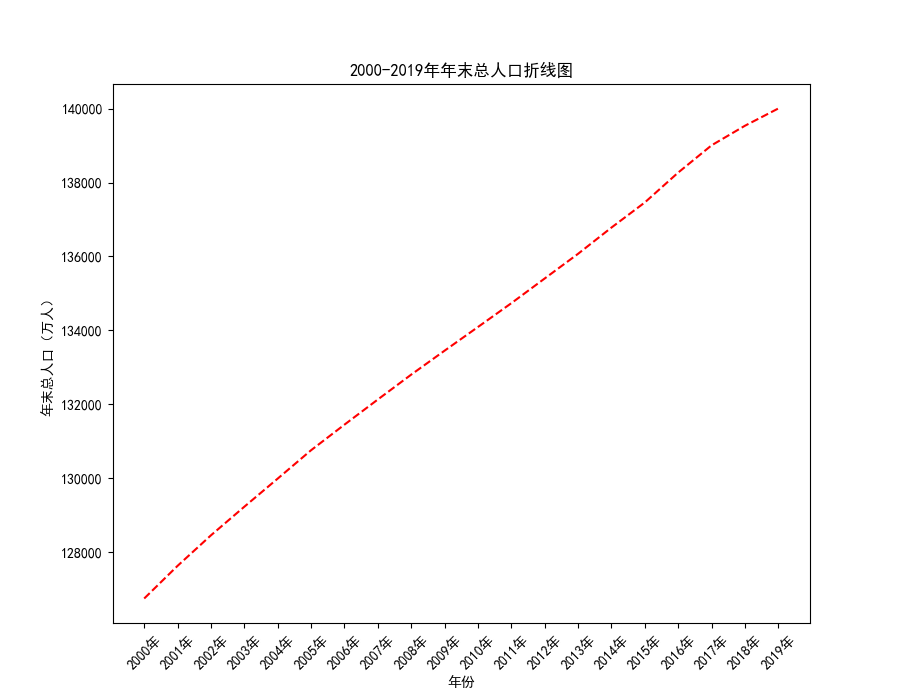
\includegraphics[width=0.6\textwidth]{part/图形化/Matplotlib/pic/绘图/2000-2019年年末总人口折线图.png}
    \caption{2000-2019年年末总人口折线图}
\end{figure}


\subsection{plt.scatter 散点图}
\codeinline{plt.scatter()} 用于绘制散点图，允许设置点的大小、颜色、形状等属性。
\begin{lstlisting}[style=demostyle,numbers=none]
scatter(x, y, s=None, c=None, marker=None, cmap=None, norm=None, vmin=None, vmax=None,
        alpha=None, linewidths=None, verts=None, edgecolors=None,
        hold=None, data=None, **kwargs)
# 参数说明：
# x : x坐标
# y : y坐标
# s : 点的大小
# c : 点的颜色
# marker : 点的形状
# cmap : 颜色映射表
# alpha : 透明度
# edgecolors : 点的边缘颜色
\end{lstlisting}

\begin{lstlisting}[style=pythonstyle]
import matplotlib.pyplot as plt
import numpy as np

# 数据
x = np.random.rand(50)
y = np.random.rand(50)
sizes = np.random.rand(50) * 1000  # 点的大小
colors = np.random.rand(50)        # 点的颜色

# 绘制散点图
plt.scatter(x, y, s=sizes, c=colors, alpha=0.6, cmap='viridis')
plt.colorbar()  # 添加颜色条
plt.title('散点图示例')
plt.show()
\end{lstlisting}

\begin{lstlisting}[style=pythonstyle]
import numpy as np
import pandas as pd
import matplotlib.pyplot as plt
plt.rcParams['font.sans-serif'] =' SimHei'
# 设置中文显示
plt.rcParams['axes.unicode_minus'] = False
data = pd.read_csv('../data/people.csv')
name = data.columns  # 提取其中的columns字段，视为数据的标签
values = data.values  # 提取其中的values字段，数据的存在位置    
plt.figure(figsize=(9, 7))  # 设置画布
plt.scatter(values[:, 0], values[:, 2], marker='o', c='red')   # 选取values中的第一列和第三列数据绘制散点图
plt.scatter(values[:, 0], values[:, 3], marker='D', c='blue')  # 选取values中的第一列和第四列数据绘制散点图
plt.scatter(values[:, 0], values[:, 4], marker='v', c='black') # 选取values中的第一列和第五列数据绘制散点图
plt.xlabel('年份')  # 添加横轴标签
plt.ylabel('年末总人口（万人）')  # 添加纵轴标签
plt.xticks(range(0, 20), values[range(0, 20), 0], rotation=45)
plt.title('2000-2019年各年龄段年末总人口散点图')  # 添加图表标题
plt.legend(['0-14岁人口', '15-64岁人口', '65岁及以上人口'])  #添加图例
plt.savefig('../tmp/2000-2019年各年龄段年末总人口散点图.png')
plt.show()
\end{lstlisting}
\begin{figure}[htpb]
    \centering
    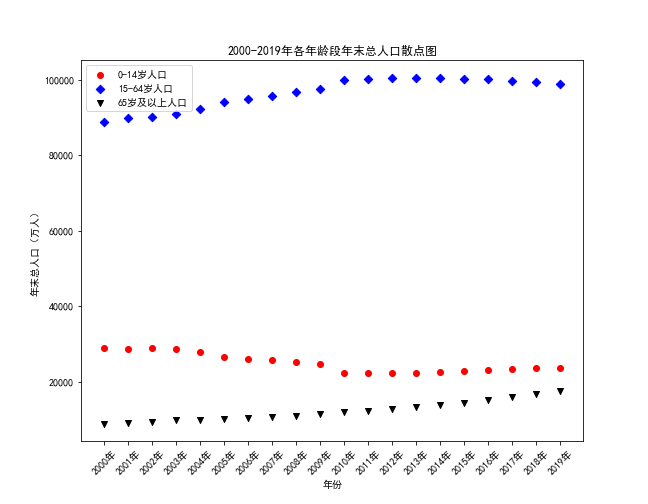
\includegraphics[width=0.5\textwidth]{part/图形化/Matplotlib/pic/绘图/2000-2019年各年龄段年末总人口数散点图.png}
    \caption{2000-2019年各年龄段年末总人口数散点图}
\end{figure}


\begin{lstlisting}[style=pythonstyle]
import matplotlib.pyplot as plt
import numpy as np

def scatter_create_color_graph():
    """
    绘制不同颜色值的散点图。
    x, y: 散点的坐标
    c: 颜色值（以十六进制表示）
    """
    x = [i for i in range(20)]
    y = [i for i in range(20)]

    plt.xticks(x)
    plt.yticks(y)
    c = np.linspace(0, 0xffffff, 20, endpoint=False)
    plt.scatter(x, y, c=c, s=200, marker='o')
    plt.title('不同颜色值绘制的散点图')

def scatter_create_markers_graph():
    """
    绘制不同标记大小和颜色的散点图。
    marker: 标记类型
    s: 标记大小
    c: 标记颜色
    """
    x = np.array([i for i in range(20)])
    y = np.array([i for i in range(20)])

    plt.xticks(x)
    plt.yticks(y)
    plt.scatter(x, y, c='orange', s=200, marker='v')
    plt.scatter(x + 1, y, c='gray', s=100, marker='^')
    plt.title('不同标记大小和颜色绘制的散点图')

def scatter_create_size_graph():
    """
    根据坐标调整标记大小的散点图。
    s: 根据位置动态调整标记大小
    """
    x = np.array([i for i in range(10)])
    y = np.array([0] * len(x))
    plt.ylim(-0.5, 1.5)
    plt.yticks([0, 1])
    plt.xticks(x)

    sizes = [20 * (n + 1) ** 2 for n in range(len(x))]
    plt.scatter(x, y, c='m', s=sizes)

    sizes = [20 * (10 - n) ** 2 for n in range(len(x))]
    plt.scatter(x, y + 1, c='m', s=sizes)
    plt.title('根据坐标调整标记大小')

def scatter_create_random_graph():
    """
    随机坐标散点图。
    x, y: 随机生成的坐标
    marker: 标记类型
    s: 标记大小
    alpha: 标记透明度
    """
    x = np.random.randn(100)
    y = np.random.randn(100)

    plt.scatter(x, y, c='m', marker='p', s=500, alpha=0.6)
    plt.title('随机坐标散点图')

def scatter_create_guess_graph():
    """
    多元高斯分布二维图。
    s: 根据分布值调整标记大小
    alpha: 标记透明度
    """
    mu_vec = np.array([0,0])
    cov_mat = np.array([[1,0],[0,1]])
    X = np.random.multivariate_normal(mu_vec, cov_mat, 1000)
    R = X ** 2
    R_sum = R.sum(axis = 1)

    plt.scatter(X[:,0], X[:,1], color='m', marker='o',
                s = 32.*R_sum, edgecolor='black', alpha=0.5)
    plt.title('多元高斯分布二维图')

def scatter_create_gradual_graph():
    """
    绘制同点渐变晕化效果。
    c: 渐变颜色值
    s: 标记大小
    """
    c = np.linspace(0xffff00, 0xffffff, 20, endpoint=False)
    for i in range(19,-1,-1):
        size = i * 10000 + 10
        cval = hex(int(c[i]))[2:]
        color = "#" + '0' * (6 - len(cval)) + cval
        plt.scatter(0, 0, s=size, c=color)
    plt.title('同点渐变晕化')

# 创建3x2的子图布局
plt.figure(figsize=(15, 10))

# 绘制每个子图
plt.subplot(3, 2, 1)
scatter_create_color_graph()

plt.subplot(3, 2, 2)
scatter_create_markers_graph()

plt.subplot(3, 2, 3)
scatter_create_size_graph()

plt.subplot(3, 2, 4)
scatter_create_random_graph()

plt.subplot(3, 2, 5)
scatter_create_guess_graph()

plt.subplot(3, 2, 6)
scatter_create_gradual_graph()

# 调整布局并显示图像
plt.tight_layout()
plt.show()   
\end{lstlisting}

\begin{figure}[htpb]
    \centering
    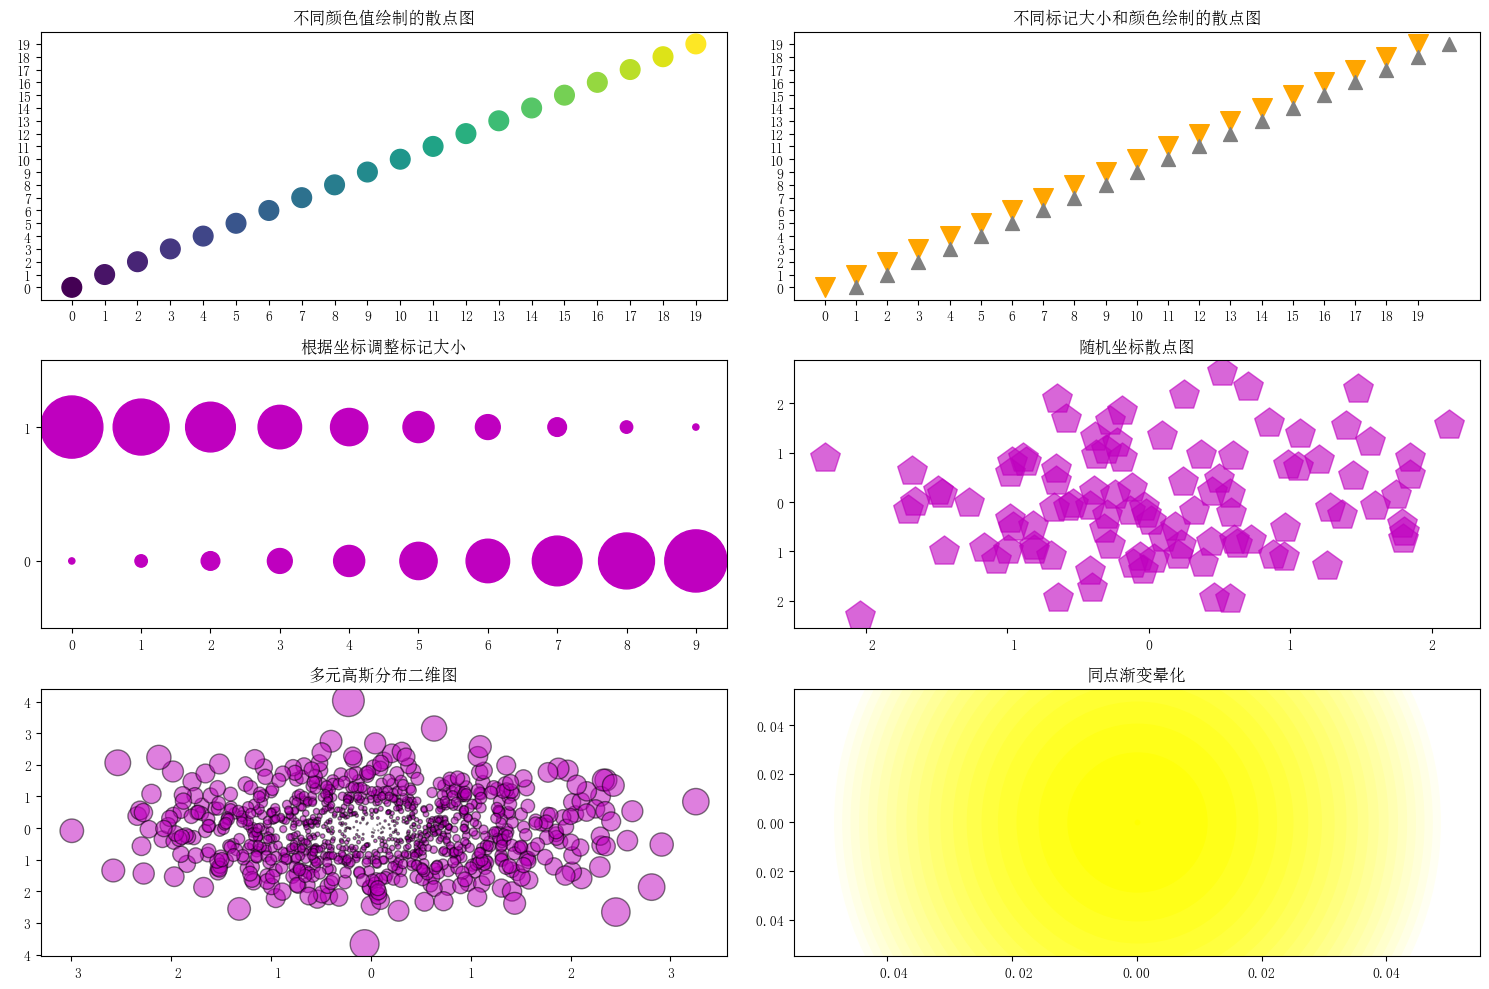
\includegraphics[width=0.6\textwidth]{part/图形化/Matplotlib/pic/绘图/不同scatter属性演示.png}
    \caption{不同scatter属性演示}
\end{figure}

\section{条形图/柱形图}
\subsection{plt.bar 垂直条形图}
\codeinline{plt.bar()} 用于绘制垂直的条形图。
\begin{lstlisting}[style=demostyle,numbers=none]
# 必须导入的库
import matplotlib.pyplot as plt
# bar 功能：绘制垂直条形图
plt.bar(x, height, width=0.8, bottom=None, align='center', **kwargs)
# 参数说明：
# x : 条形的 x 坐标
# height : 条形的高度
# width : 条形的宽度
# bottom : 条形的底部位置
# align : 对齐方式
## 'center'：居中
## 'edge'：边缘对齐
\end{lstlisting}

\begin{lstlisting}[style=pythonstyle]
import matplotlib.pyplot as plt

# 数据
categories = ['A', 'B', 'C', 'D']
values = [10, 24, 36, 12]

# 绘制垂直条形图
plt.bar(categories, values, color='skyblue')
plt.title('垂直条形图')
plt.show()
\end{lstlisting}
\begin{figure}[htpb]
    \centering
    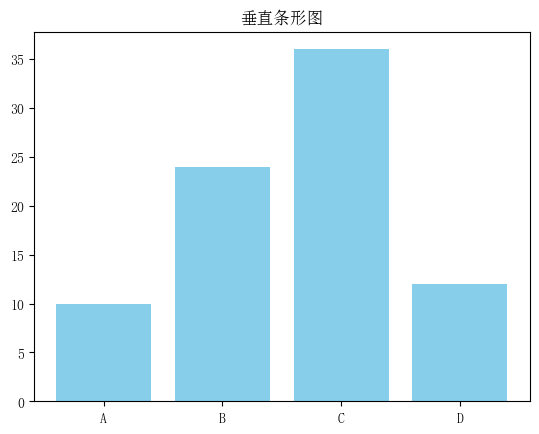
\includegraphics[width=0.6\textwidth]{part/图形化/Matplotlib/pic/绘图/垂直条形图.png}
    \caption{垂直条形图}
\end{figure}


\subsection{plt.bar 堆叠条形图}
\codeinline{plt.bar()} 可以通过设置底部来实现堆叠条形图。
\begin{lstlisting}[style=pythonstyle]
import matplotlib.pyplot as plt

# 数据
categories = ['A', 'B', 'C', 'D']
values1 = [10, 20, 30, 40]
values2 = [5, 15, 25, 10]

# 绘制堆叠条形图
plt.bar(categories, values1, color='lightblue', label='Values 1')
plt.bar(categories, values2, bottom=values1, color='orange', label='Values 2')
plt.title('堆叠条形图')
plt.legend()
plt.show()
\end{lstlisting}

\begin{figure}[htpb]
    \centering
    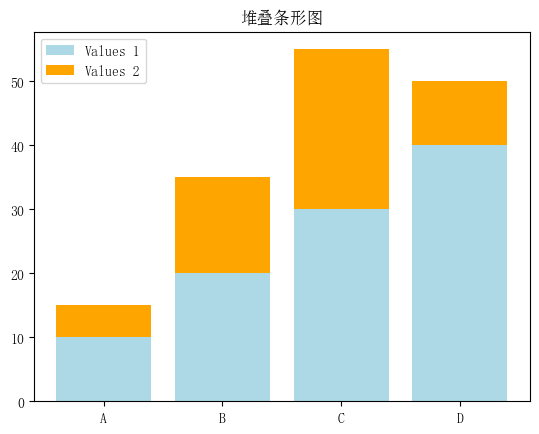
\includegraphics[width=0.6\textwidth]{part/图形化/Matplotlib/pic/绘图/堆叠条形图.png}
    \caption{堆叠条形图}
\end{figure}


\subsection{plt.bar 并列条形图}
并列条形图可以通过调整条形的宽度和位置来实现。
\begin{lstlisting}[style=pythonstyle]
import matplotlib.pyplot as plt
import numpy as np

# 数据
categories = np.arange(4)
values1 = [10, 20, 30, 40]
values2 = [5, 15, 25, 10]

# 绘制并列条形图
plt.bar(categories - 0.2, values1, width=0.4, color='lightblue', label='Values 1')
plt.bar(categories + 0.2, values2, width=0.4, color='orange', label='Values 2')
plt.title('并列条形图')
plt.legend()
plt.show()
\end{lstlisting}
\begin{figure}[htpb]
    \centering
    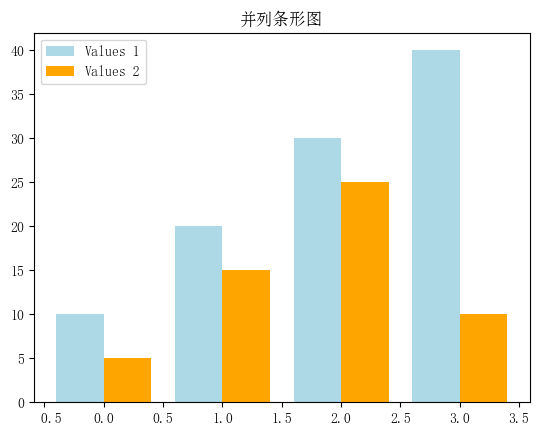
\includegraphics[width=0.6\textwidth]{part/图形化/Matplotlib/pic/绘图/并列条形图.png}
    \caption{并列条形图}
\end{figure}


\subsection{plt.barh 水平条形图}
\codeinline{plt.barh()} 用于绘制水平条形图。
\begin{lstlisting}[style=demostyle,numbers=none]
# 必须导入的库
import matplotlib.pyplot as plt
# barh 功能：绘制水平条形图
plt.barh(y, width, height=0.8, left=None, align='center', **kwargs)
# 参数说明：
# y : 条形的 y 坐标
# width : 条形的宽度
# height : 条形的高度
# left : 条形的左侧位置
# align : 对齐方式
## 'center'：居中
## 'edge'：边缘对齐
\end{lstlisting}
\begin{lstlisting}[style=pythonstyle]
import matplotlib.pyplot as plt

# 数据
categories = ['A', 'B', 'C', 'D']
values = [10, 24, 36, 12]

# 绘制水平条形图
plt.barh(categories, values, color='skyblue')
plt.title('水平条形图')
plt.show()
\end{lstlisting}
\begin{figure}[htpb]
    \centering
    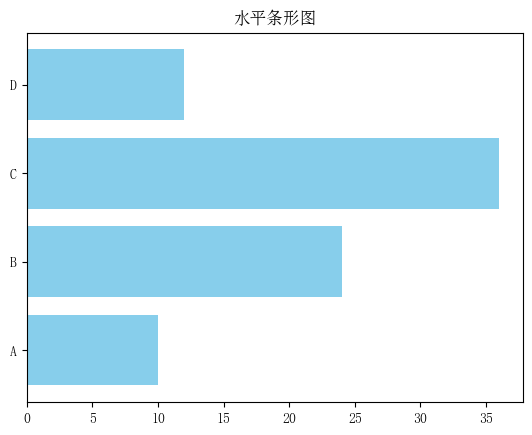
\includegraphics[width=0.6\textwidth]{part/图形化/Matplotlib/pic/绘图/水平条形图.png}
    \caption{水平条形图}
\end{figure}


% \section{折线图}
% \label{sec:matplotlib_line}
% \codeinline{plt.plot()} 用于绘制折线图。
% \begin{lstlisting}[style=pythonstyle]
% import matplotlib.pyplot as plt
% import numpy as np

% # 数据
% x = np.linspace(0, 10, 100)
% y = np.sin(x)

% # 绘制折线图
% plt.plot(x, y, color='green', linewidth=2, linestyle='--')
% plt.title('折线图')
% plt.show()
% \end{lstlisting}

\section{pie 饼图}
\codeinline{plt.pie()} 用于绘制饼图。
\begin{lstlisting}[style=demostyle,numbers=none]
# 必须导入的库
import matplotlib.pyplot as plt
# pie 功能：绘制饼图
plt.pie(x, explode=None, labels=None, colors=None, autopct=None, pctdistance=0.6, **kwargs)
# 参数说明：
# x : 每个饼块的大小
# explode : 是否突出显示饼块
# labels : 饼块的标签
# colors : 饼块的颜色
# autopct : 显示百分比的格式
# pctdistance : 标签距离圆心的比例
\end{lstlisting}
\begin{lstlisting}[style=pythonstyle]
import matplotlib.pyplot as plt

# 数据
sizes = [15, 30, 45, 10]
labels = ['A', 'B', 'C', 'D']
colors = ['gold', 'yellowgreen', 'lightcoral', 'lightskyblue']

# 绘制饼图
plt.pie(sizes, labels=labels, colors=colors, autopct='%1.1f%%', shadow=True, startangle=140)
plt.title('饼图示例')
plt.axis('equal')  # 保持圆形
plt.show()
\end{lstlisting}
\begin{figure}[htpb]
    \centering
    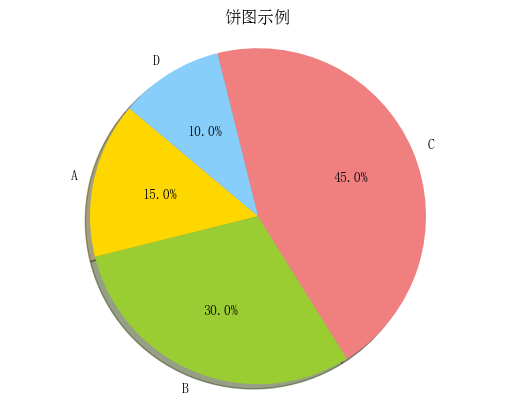
\includegraphics[width=0.6\textwidth]{part/图形化/Matplotlib/pic/绘图/饼图示例.png}
    \caption{饼图示例}
\end{figure}
\begin{lstlisting}[style=pythonstyle]
import matplotlib.pyplot as plt
labels = ['English', 'Maths', 'Chemistry']
scores = [90, 75, 88]
explode = (0, 0, 0.1) # 突出显示Chemistry
plt.pie(scores, explode=explode, labels=labels,
        autopct='%1.1f%%', shadow=True, startangle=60)
plt.axis('equal')
plt.legend(loc="upper right")
plt.title('学科成绩比例(突出显示Chemistry)')
plt.show()
\end{lstlisting}    
\begin{figure}[htpb]
    \centering
    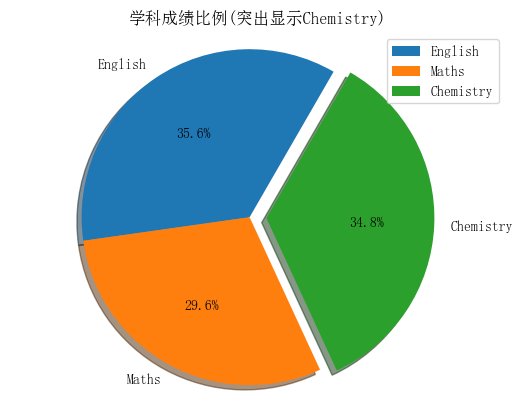
\includegraphics[width=0.6\textwidth]{part/图形化/Matplotlib/pic/绘图/学科成绩比例(突出显示Chemistry).png}
    \caption{学科成绩比例(突出显示Chemistry)}
\end{figure}

\begin{lstlisting}[style=pythonstyle]
import numpy as np
import matplotlib.pyplot as plt
import pandas as pd
plt.rcParams['font.sans-serif'] = 'SimHei'  # 设置中文显示
plt.rcParams['axes.unicode_minus'] = False

# 读取数据
data = pd.read_csv('../data/people.csv')
name = data.columns  # 提取其中的columns字段，视为数据的标签
values = data.values  # 提取其中的values字段，数据的存在位置
label = ['0-14岁人口', '15-64岁人口', '65岁及以上人口']  # 刻度标签
plt.figure(figsize=(6, 6))      # 将画布设定为正方形，则绘制的饼图是正圆

# 绘制饼图
explode = [0.01, 0.01, 0.01]    # 设定各项离心n个半径
plt.pie(values[-1, 2:5], explode=explode, labels=label, autopct='%1.1f%%')  
# values[-1, 2:5] 代表最后一行的第2、3、4列数据
# explode=explode 代表各项离心n个半径
# labels=label 代表各项标签
# autopct='%1.1f%%' 代表数值保留固定小数位

plt.title('2019年各年龄段年末总人口饼图')  # 添加图表标题
plt.savefig('../tmp/2019年各年龄段年末总人口饼图.png')
plt.show()
\end{lstlisting}
\begin{figure}[htpb]
    \centering
    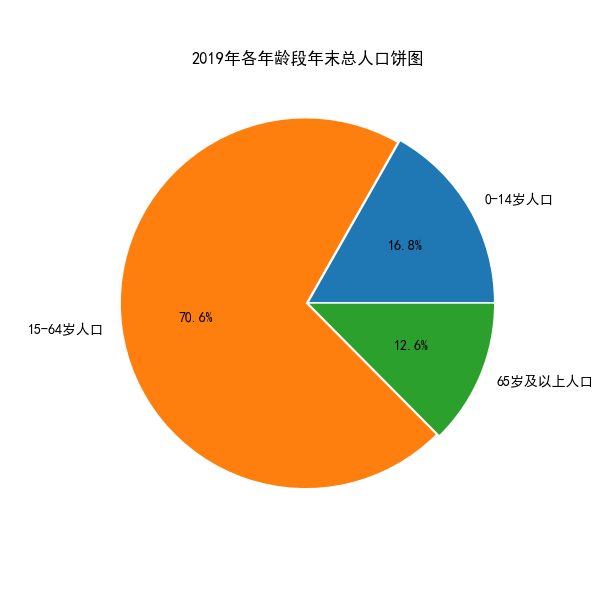
\includegraphics[width=0.4\textwidth]{part/图形化/Matplotlib/pic/绘图/2019年各年龄段年末总人口饼图.png}
    \caption{2019年各年龄段年末总人口饼图}
    \label{fig:2019年各年龄段年末总人口饼图}
\end{figure}





\section{boxplot 箱线图}
\codeinline{plt.boxplot()} 用于绘制箱线图。
\begin{lstlisting}[style=demostyle,numbers=none]
# 必须导入的库
import matplotlib.pyplot as plt
# boxplot 功能：绘制箱线图
plt.boxplot(x, notch=None, vert=None, patch_artist=None, widths=None, **kwargs)
# 参数说明：
# x : 数据
# notch : 是否为凹槽形
# vert : 是否垂直显示
# patch_artist : 是否填充箱体
# widths : 箱体的宽度
\end{lstlisting}
\begin{lstlisting}[style=pythonstyle]
import matplotlib.pyplot as plt
import numpy as np

# 数据
np.random.seed(10)
data = [np.random.normal(0, std, 100) for std in range(1, 4)]

# 绘制箱线图
plt.boxplot(data, vert=True, patch_artist=True, labels=['A', 'B', 'C'])
plt.title('箱线图')
plt.show()
\end{lstlisting}
\begin{figure}[htpb]
    \centering
    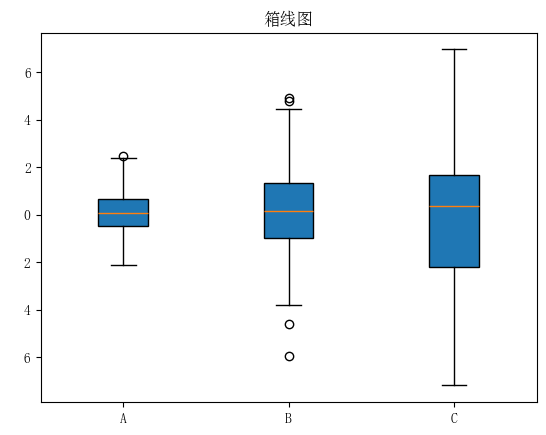
\includegraphics[width=0.6\textwidth]{part/图形化/Matplotlib/pic/绘图/箱型图演示.png}
    \caption{箱型图演示}
    \label{fig:箱型图演示}
\end{figure}

\begin{lstlisting}[style=pythonstyle]
import numpy as np
import matplotlib.pyplot as plt
import pandas as pd
plt.rcParams['font.sans-serif'] = 'SimHei'  # 设置中文显示
plt.rcParams['axes.unicode_minus'] = False
data = pd.read_csv('../data/people.csv')
name = data.columns  # 提取其中的columns字段，视为数据的标签
values = data.values  # 提取其中的values字段，数据的存在位置


label= ['0-14岁人口', '15-64岁人口', '65岁及以上人口']  # 定义标签
gdp = (list(values[:, 2]), list(values[:, 3]), list(values[:, 4]))
plt.figure(figsize=(7, 6))

# 绘制箱线图
plt.boxplot(gdp, notch=True, labels=label, meanline=True)
# notch=True 代表箱体是否为凹槽形
# labels=label 代表各项标签
# meanline=True 代表是否显示均值线

plt.title('2000-2019年各年龄段年末总人口箱线图')
plt.savefig('../tmp/2000-2019年各年龄段年末总人口箱线图.png')
plt.show()
\end{lstlisting}
\begin{figure}[htpb]
    \centering
    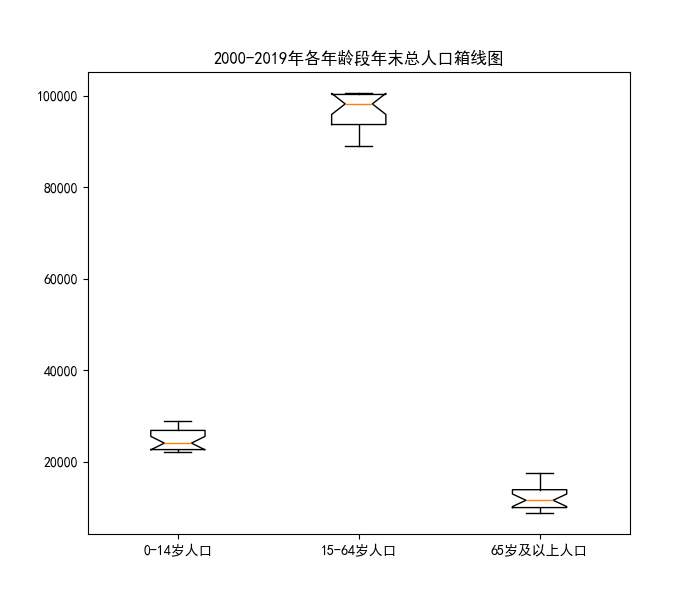
\includegraphics[width=0.4\textwidth]{part/图形化/Matplotlib/pic/绘图/2000-2019年各年龄段年末总人口箱线图.png}
    \caption{2000-2019年各年龄段年末总人口箱线图}
    \label{fig:2000-2019年各年龄段年末总人口箱线图}
\end{figure}



\section{直方图}
\subsection{plt.hist 一维频率直方图}
\begin{lstlisting}[style=demostyle,numbers=none]
# 必须导入的库
import matplotlib.pyplot as plt
# hist 功能：绘制一维频率直方图
plt.hist(x, bins=None, density=None, **kwargs)
# 参数说明：
# x : 数据
# bins : 分箱的数量或位置
# density : 是否显示概率密度
\end{lstlisting}
\codeinline{plt.hist()} 用于绘制一维频率直方图。
\begin{lstlisting}[style=pythonstyle]
import matplotlib.pyplot as plt
import numpy as np

# 数据
data = np.random.randn(1000)

# 绘制一维频率直方图
plt.hist(data, bins=30, alpha=0.7, color='blue')
plt.title('一维频率直方图')
plt.show()
\end{lstlisting}
\begin{figure}[htpb]
    \centering
    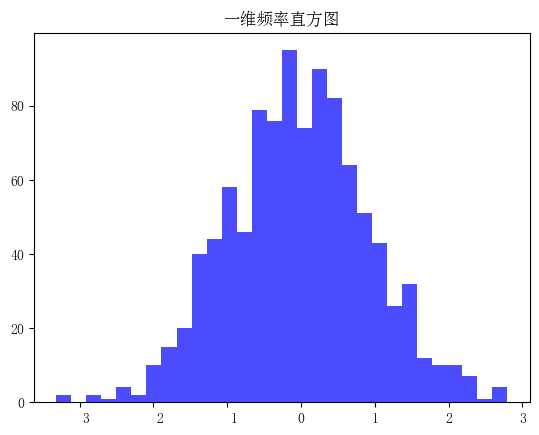
\includegraphics[width=0.6\textwidth]{part/图形化/Matplotlib/pic/绘图/一维频率直方图.png}
    \caption{一维频率直方图}
\end{figure}

\begin{lstlisting}[style=pythonstyle]
import matplotlib.pyplot as plt
import numpy as np

# 生成随机数据
data = np.random.randn(1000)

# 创建图像和子图
plt.figure(figsize=(8, 4))

# 第一个子图：histtype='step'
plt.subplot(1, 2, 1)
plt.title('step')
plt.hist(data, bins=50, density=True, alpha=1,  # density=True 代替旧的 normed=True
         histtype='step', color='grey', edgecolor='black')  # 线条模式，不填充

# 第二个子图：histtype='stepfilled'
plt.subplot(1, 2, 2)
plt.title('stepfilled')
plt.hist(data, bins=50, density=True, alpha=1, 
         histtype='stepfilled', color='grey', edgecolor='none')  # 填充的模式

# 调整布局并显示图像
plt.tight_layout()
plt.show()
\end{lstlisting}

\begin{figure}[htpb]
    \centering
    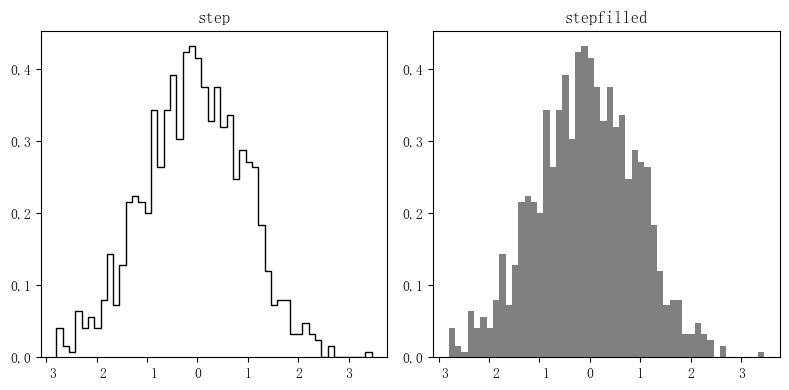
\includegraphics[width=0.6\textwidth]{part/图形化/Matplotlib/pic/绘图/不同histtype类型的直方图.png}
    \caption{不同histtype类型的直方图}
\end{figure}

stepfilled 与透明性参数 alpha 搭配使用的效果非常好：
\begin{lstlisting}[style=pythonstyle]
import matplotlib.pyplot as plt
import numpy as np

# 生成随机数据
x1 = np.random.normal(0, 2, 1000)    # 均值为0，标准差为2的正态分布
x2 = np.random.normal(-2, 1, 1000)   # 均值为-2，标准差为1的正态分布
x3 = np.random.normal(2, 2, 1000)    # 均值为2，标准差为2的正态分布

# 设置直方图的样式参数
kwargs = dict(histtype='stepfilled', alpha=0.5, density=True, bins=40)

# 创建图像
plt.figure(figsize=(8, 4))

# 绘制直方图
plt.hist(x1, **kwargs, color='blue', label='x1')  # 第一个数据集
plt.hist(x2, **kwargs, color='orange', label='x2')  # 第二个数据集
plt.hist(x3, **kwargs, color='green', label='x3')  # 第三个数据集

# 添加图例
plt.legend()

# 显示图像
plt.title('不同透明度的频次直方图')
plt.show()
\end{lstlisting}
\begin{figure}[htpb]
    \centering
    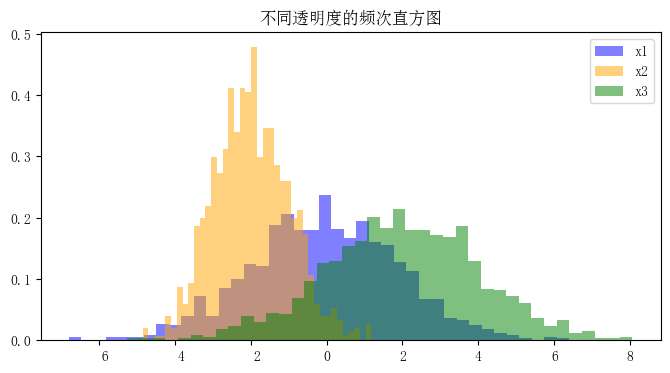
\includegraphics[width=0.6\textwidth]{part/图形化/Matplotlib/pic/绘图/不同透明度的频次直方图.png}
    \caption{不同透明度的频次直方图}
\end{figure}



\subsection{plt.hist2d 二维频率直方图}
\codeinline{plt.hist2d()} 用于绘制二维频率直方图。
\begin{lstlisting}[style=demostyle,numbers=none]
# 必须导入的库
import matplotlib.pyplot as plt
# hist2d 功能：绘制二维频率直方图
plt.hist2d(x, y, bins=10, range=None, density=False, cmap=None, **kwargs)
# 参数说明：
# x : x坐标
# y : y坐标
# bins : 分箱数
# range : x 和 y 的值范围
# density : 是否归一化
# cmap : 颜色映射
\end{lstlisting}
\begin{lstlisting}[style=pythonstyle]
import matplotlib.pyplot as plt
import numpy as np

# 数据
x = np.random.randn(1000)
y = np.random.randn(1000)

# 绘制二维频率直方图
plt.hist2d(x, y, bins=30, cmap='Blues')
plt.colorbar()
plt.title('二维频率直方图')
plt.show()
\end{lstlisting}
\begin{figure}[htpb]
    \centering
    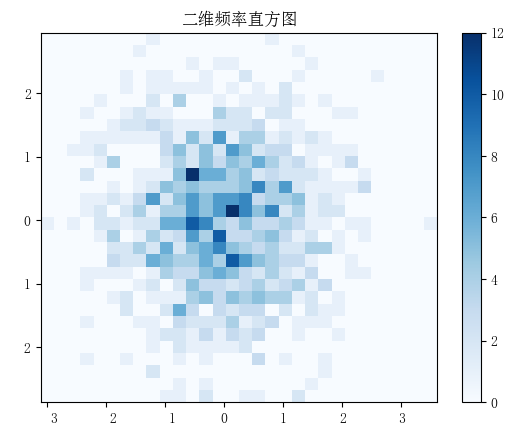
\includegraphics[width=0.6\textwidth]{part/图形化/Matplotlib/pic/绘图/二维频率直方图.png}
    \caption{二维频率直方图}
\end{figure}


\subsection{plt.hexbin 六边形区间划分}
二维频次直方图是由与坐标轴正交的方块分割而成的， 还有一种常用的方式是用正六边形分割。
\codeinline{plt.hexbin()} 用于绘制六边形区间划分。
\begin{lstlisting}[style=demostyle,numbers=none]
# 必须导入的库
import matplotlib.pyplot as plt
# hexbin 功能：绘制六边形分箱图
plt.hexbin(x, y, gridsize=30, cmap=None, **kwargs)
# 参数说明：
# x : x坐标
# y : y坐标
# gridsize : 网格大小
# cmap : 颜色映射
\end{lstlisting}
\begin{lstlisting}[style=pythonstyle]
import matplotlib.pyplot as plt
import numpy as np

# 数据
x = np.random.randn(10000)
y = np.random.randn(10000)

# 绘制六边形区间划分
plt.hexbin(x, y, gridsize=30, cmap='Greens')
plt.colorbar()
plt.title('六边形区间划分')
plt.show()
\end{lstlisting}
\begin{figure}[htpb]
    \centering
    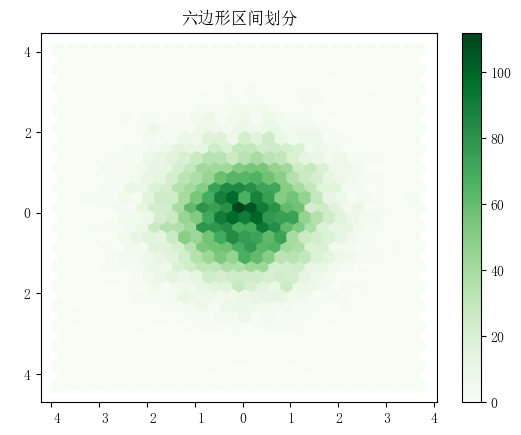
\includegraphics[width=0.6\textwidth]{part/图形化/Matplotlib/pic/绘图/六边形区间划分.png}
    \caption{六边形区间划分}
\end{figure}


\section{imshow热力图}
\codeinline{plt.imshow()} 用于绘制热力图。
\begin{lstlisting}[style=demostyle,numbers=none]
# 必须导入的库
import matplotlib.pyplot as plt
# imshow 功能：显示图像数据
plt.imshow(X, cmap=None, interpolation=None, **kwargs)
# 参数说明：
# X : 图像数据
# cmap : 颜色映射
# interpolation : 插值方法
## 'nearest'：最近邻插值
## 'bilinear'：双线性插值
## 'bicubic'：双三次插值
\end{lstlisting}
\begin{lstlisting}[style=pythonstyle]
import matplotlib.pyplot as plt
import numpy as np

# 数据
data = np.random.rand(10, 10)

# 绘制热力图
plt.imshow(data, cmap='hot', interpolation='nearest')
plt.colorbar()
plt.title('热力图')
plt.show()
\end{lstlisting}

\section{等高线图}
\subsection{plt.contour 等高线图}
\codeinline{plt.contour()} 用于绘制等高线图。
\begin{lstlisting}[style=demostyle,numbers=none]
# 必须导入的库
import matplotlib.pyplot as plt
# contour 功能：绘制等高线图
plt.contour(X, Y, Z, levels=None, colors=None, **kwargs)
# 参数说明：
# X, Y : 网格坐标
# Z : 等高线数据
# levels : 等高线的层次
# colors : 线条颜色
\end{lstlisting}
\begin{lstlisting}[style=pythonstyle]
import matplotlib.pyplot as plt
import numpy as np

# 数据
x = np.linspace(-3.0, 3.0, 100)
y = np.linspace(-3.0, 3.0, 100)
X, Y = np.meshgrid(x, y)
Z = np.exp(-X**2 - Y**2)

# 绘制等高线图
plt.contour(X, Y, Z, levels=10, cmap='viridis') # levels=10 表示等高线的数量 cmaps='viridis' 表示颜色
plt.title('等高线图')
plt.show()
\end{lstlisting}
\begin{figure}[htpb]
    \centering
    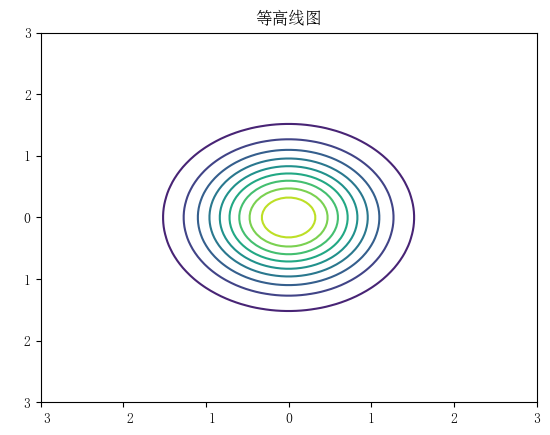
\includegraphics[width=0.6\textwidth]{part/图形化/Matplotlib/pic/绘图/等高线图-level10camaps=viridis.png}
    \caption{level=10,camaps=viridis的等高线图}
\end{figure}

\begin{lstlisting}[style=pythonstyle]
import matplotlib.pyplot as plt
import numpy as np

# 定义函数 f(x, y)
def f(x, y):
    return np.sin(x) ** 10 + np.cos(10 + y * x)

# 设置绘图风格
# plt.style.use('seaborn-v0_8-white')
plt.rcParams['font.family'] = 'SimSun'   

# 生成数据
x = np.linspace(0, 5, 50)
y = np.linspace(0, 5, 40)
X, Y = np.meshgrid(x, y)
Z = f(X, Y)

# 绘制等高线图
plt.contour(X, Y, Z, colors='black')

# 显示图像
plt.title('等高线图')
plt.show()
\end{lstlisting}

\begin{figure}[htpb]
    \centering
    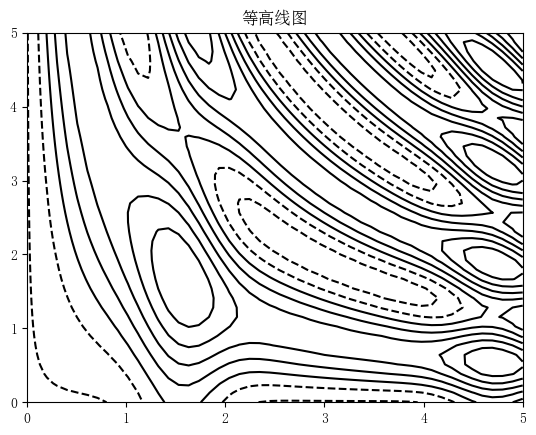
\includegraphics[width=0.6\textwidth]{part/图形化/Matplotlib/pic/绘图/实线和虚线是通过默认的等高线分布自动生成的.png}
    \caption{实线和虚线是通过默认的等高线分布自动生成的}
\end{figure}

实线：通常表示正值等高线的部分，代表函数在这些区域内的高度（或值）大于某一基准值。

虚线：通常表示负值等高线的部分，代表函数在这些区域内的高度（或值）小于某一基准值。

\begin{lstlisting}[style=pythonstyle]
import matplotlib.pyplot as plt
import numpy as np

# 定义函数 f(x, y)
def f(x, y):
    return np.sin(x) ** 10 + np.cos(10 + y * x)

# 生成数据
x = np.linspace(0, 5, 50)
y = np.linspace(0, 5, 40)
X, Y = np.meshgrid(x, y)
Z = f(X, Y)

# 绘制等高线图，并等分为20份，使用copper颜色方案
plt.contour(X, Y, Z, 20, cmap='copper')

# 显示图像
plt.title('使用copper色彩方案的等高线图')
plt.show()
\end{lstlisting}
\begin{figure}[htpb]
    \centering
    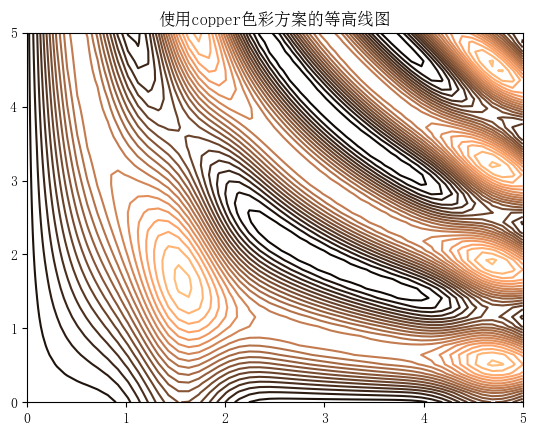
\includegraphics[width=0.6\textwidth]{part/图形化/Matplotlib/pic/绘图/使用copper色彩方案的等高线图.png}
    \caption{使用copper色彩方案的等高线图}
\end{figure}




\subsection{plt.contourf 带填充色的等高线图}
\codeinline{plt.contourf()} 用于绘制带填充色的等高线图。
\begin{lstlisting}[style=demostyle,numbers=none]
# 必须导入的库
import matplotlib.pyplot as plt
# contourf 功能：绘制填充的等高线图
plt.contourf(X, Y, Z, levels=None, cmap=None, **kwargs)
# 参数说明：
# X, Y : 网格坐标
# Z : 等高线数据
# levels : 等高线的层次
# cmap : 颜色映射
\end{lstlisting}
\begin{lstlisting}[style=pythonstyle]
import matplotlib.pyplot as plt
import numpy as np

# 定义函数 f(x, y)
def f(x, y):
    return np.sin(x) ** 10 + np.cos(10 + y * x)

# 生成数据
x = np.linspace(0, 5, 50)
y = np.linspace(0, 5, 40)
X, Y = np.meshgrid(x, y)
Z = f(X, Y)

# 绘制填充的等高线图，并等分为20份，使用copper颜色方案
plt.contourf(X, Y, Z, 20, cmap='copper')

# 添加颜色条
plt.colorbar()

# 显示图像
plt.title('颜色填充的等高线图')
plt.show()
\end{lstlisting}
\begin{figure}[htpb]
    \centering
    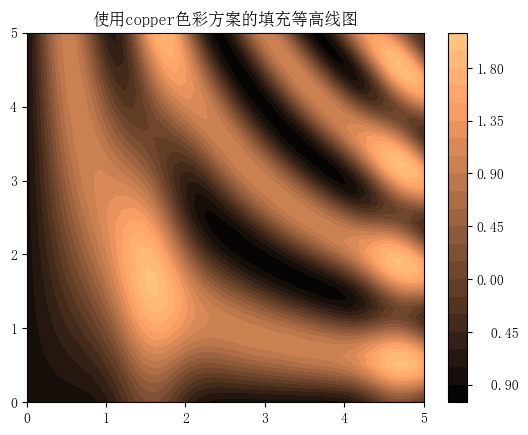
\includegraphics[width=0.6\textwidth]{part/图形化/Matplotlib/pic/绘图/颜色填充的等高线图.png}
    \caption{颜色填充的等高线图}
    \label{fig:颜色填充的等高线图}
\end{figure}

\begin{lstlisting}[style=pythonstyle]
import matplotlib.pyplot as plt
import numpy as np

# 定义函数 f(x, y)
def f(x, y):
    return np.sin(x) ** 10 + np.cos(10 + y * x)

# 生成数据
x = np.linspace(0, 5, 50)
y = np.linspace(0, 5, 40)
X, Y = np.meshgrid(x, y)
Z = f(X, Y)

# 绘制填充的等高线图，使用 hot 颜色方案，透明度为 0.75
plt.contourf(X, Y, Z, 20, alpha=0.75, cmap='hot')

# 画等高线，设置为黑色，线宽为 0.5
contours = plt.contour(X, Y, Z, 5, colors='black', linewidths=0.5)

# 为等高线添加标签
plt.clabel(contours, inline=True, fontsize=10)

# 添加颜色条
plt.colorbar()

# 显示图像
plt.title('使用 hot 色彩方案并添加标签的等高线图')
plt.show()
\end{lstlisting}
\begin{figure}[htpb]
    \centering
    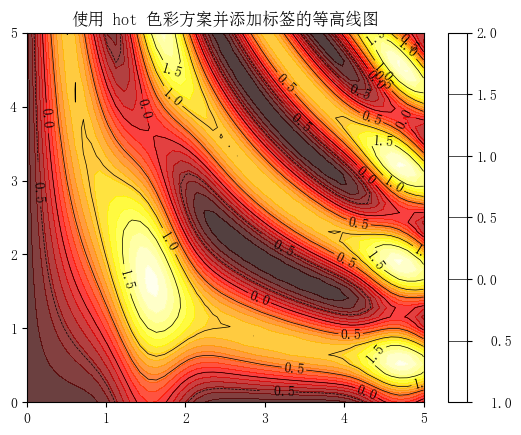
\includegraphics[width=0.6\textwidth]{part/图形化/Matplotlib/pic/绘图/使用hot色彩方案并添加标签的等高线图.png}
    \caption{使用hot色彩方案并添加标签的等高线图}
\end{figure}


\section{三维图}
Matplotlib 原本只能画2D图，后来扩展了 mplot3d 工具箱，它用来画三维图。
\begin{lstlisting}[style=demostyle,numbers=none]
from mpl_toolkits import mplot3d
# 或
from mpl_toolkits.mplot3d import Axes3D
\end{lstlisting} 

\subsection{plt.plot3D 三维数据点与线}
\codeinline{plt.plot3D()} 用于绘制三维数据点与线。
\begin{lstlisting}[style=demostyle,numbers=none]
# 必须导入的库
import matplotlib.pyplot as plt
from mpl_toolkits.mplot3d import Axes3D
# plot3D 功能：绘制三维数据点与线
plt.plot3D(x, y, z, color=None, **kwargs)
# 参数说明：
# x, y, z : 三维坐标
# color : 线条颜色
\end{lstlisting}
\begin{lstlisting}[style=pythonstyle]
import matplotlib.pyplot as plt
import numpy as np
from mpl_toolkits.mplot3d import Axes3D

# 数据
z = np.linspace(0, 1, 100)
x = z * np.sin(25 * z)
y = z * np.cos(25 * z)

# 绘制三维数据点与线
fig = plt.figure()
ax = fig.add_subplot(111, projection='3d')
ax.plot3D(x, y, z, 'gray')
plt.title(r'三维数据点与线 $x=z \cdot \sin(25z)$, $y=z \cdot \cos(25z)$')
plt.show()
\end{lstlisting}
\begin{figure}[htpb]
    \centering
    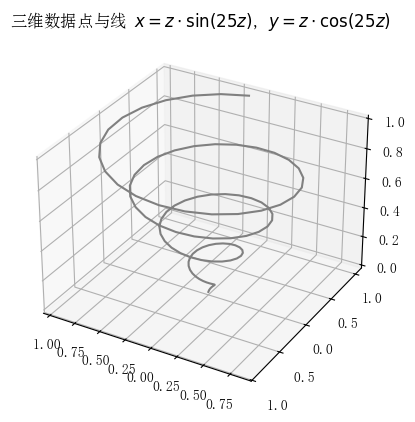
\includegraphics[width=0.6\textwidth]{part/图形化/Matplotlib/pic/绘图/三维数据点与线演示1.png}
    \caption{三维数据点与线 $x=z \cdot \sin(25z)$, $y=z \cdot \cos(25z)$}
    \label{fig:三维数据点与线演示1}
\end{figure}


\subsection{plt.contour3D 三维等高线图}
\codeinline{plt.contour3D()} 用于绘制三维等高线图。
\begin{lstlisting}[style=demostyle,numbers=none]
# 必须导入的库
import matplotlib.pyplot as plt
from mpl_toolkits.mplot3d import Axes3D
# contour3D 功能：绘制三维等高线图
plt.contour3D(X, Y, Z, levels=None, cmap=None, **kwargs)
# 参数说明：
# X, Y, Z : 三维网格数据
# levels : 等高线层数
# cmap : 颜色映射
\end{lstlisting}
\begin{lstlisting}[style=demostyle,numbers=none]
# contour3D()函数用法
ax.contour3D(X, Y, Z, 50, cmap='binary')
\end{lstlisting}

\begin{lstlisting}[style=pythonstyle]
import matplotlib.pyplot as plt
import numpy as np
from mpl_toolkits.mplot3d import Axes3D

# 数据
x = np.linspace(-3, 3, 100)
y = np.linspace(-3, 3, 100)
X, Y = np.meshgrid(x, y)
Z = np.sin(np.sqrt(X**2 + Y**2))

# 绘制三维等高线图
fig = plt.figure()
ax = fig.add_subplot(111, projection='3d')
ax.contour3D(X, Y, Z, 50, cmap='binary')
plt.title('三维等高线图')
plt.show()
\end{lstlisting}

\begin{lstlisting}[style=pythonstyle]
import matplotlib.pyplot as plt
import numpy as np
from mpl_toolkits.mplot3d import Axes3D

# 定义数据
x = np.linspace(-6, 6, 50)
y = np.linspace(-6, 6, 50)
X, Y = np.meshgrid(x, y)
Z = np.sin(np.sqrt(X**2 + Y**2))

# 定义绘图函数
def draw(ax, X, Y, Z):
    ax.contour3D(X, Y, Z, 40, cmap='hot')
    ax.set_xlabel('x')
    ax.set_ylabel('y')
    ax.set_zlabel('z')

# 创建图形和子图
fig = plt.figure(figsize=(10, 8))

# 第一个子图，默认视角
ax1 = fig.add_subplot(2, 2, 1, projection='3d')
draw(ax1, X, Y, Z)

# 第二个子图，调整俯仰角和方位角
ax2 = fig.add_subplot(2, 2, 2, projection='3d')
draw(ax2, X, Y, Z)
ax2.view_init(60, 35)  # 调整俯仰角为60度，方位角为35度

# 第三个子图，调整为俯视角度
ax3 = fig.add_subplot(2, 2, 3, projection='3d')
draw(ax3, X, Y, Z)
ax3.view_init(-90, 0)  # 调整俯仰角为-90度

# 第四个子图，反向视角
ax4 = fig.add_subplot(2, 2, 4, projection='3d')
draw(ax4, X, Y, Z)
ax4.view_init(-180, 35)  # 反方向，调整为-180度的俯仰角

# 调整布局并显示图像
plt.tight_layout()
plt.show()
\end{lstlisting}
\begin{figure}[htpb]
    \centering
    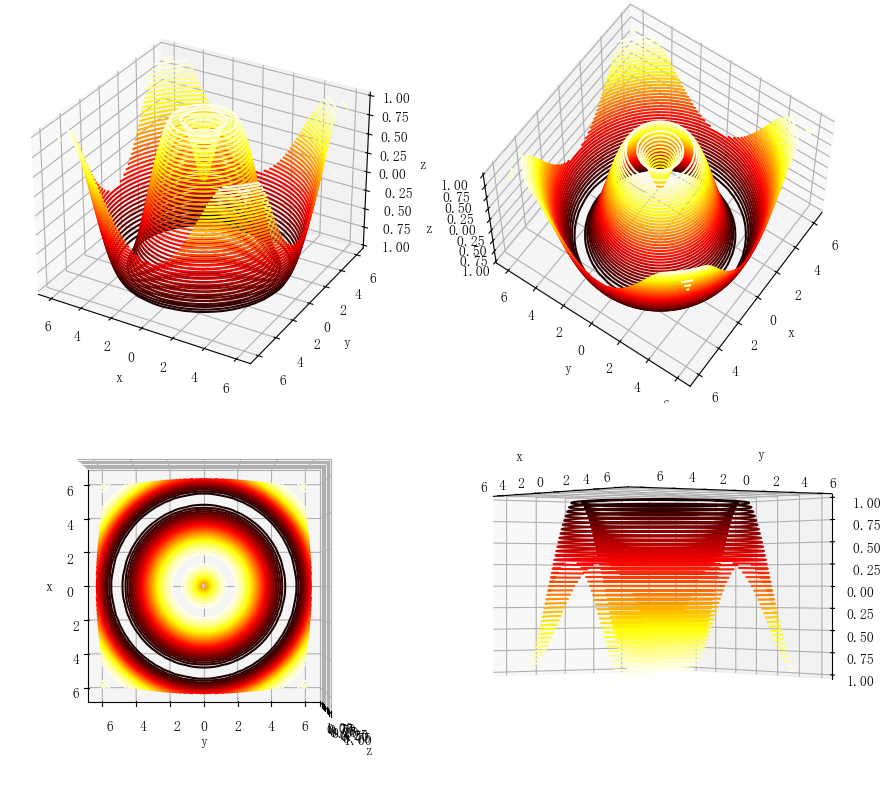
\includegraphics[width=0.8\textwidth]{part/图形化/Matplotlib/pic/绘图/3D等高线不同视图.png}
    \caption{3D等高线不同视图}
    \label{fig:3D等高线不同视图}
\end{figure}



\subsection{plt.plot\_wireframe 线框图}
\codeinline{plt.plot\_wireframe()} 用于绘制线框图。
\begin{lstlisting}[style=demostyle,numbers=none]
# 必须导入的库
import matplotlib.pyplot as plt
from mpl_toolkits.mplot3d import Axes3D
# plot_wireframe 功能：绘制线框图
plt.plot_wireframe(X, Y, Z, rstride=1, cstride=1, **kwargs)
# 参数说明：
# X, Y, Z : 网格数据
# rstride : 行步长
# cstride : 列步长
\end{lstlisting}
\begin{lstlisting}[style=pythonstyle]
import matplotlib.pyplot as plt
import numpy as np
from mpl_toolkits.mplot3d import Axes3D

# 数据
x = np.linspace(-5, 5, 50)
y = np.linspace(-5, 5, 50)
X, Y = np.meshgrid(x, y)
Z = np.sin(np.sqrt(X**2 + Y**2))

# 绘制线框图
fig = plt.figure()
ax = fig.add_subplot(111, projection='3d')
ax.plot_wireframe(X, Y, Z, color='black')
plt.title('线框图')
plt.show()
\end{lstlisting}
\begin{figure}[htpb]
    \centering
    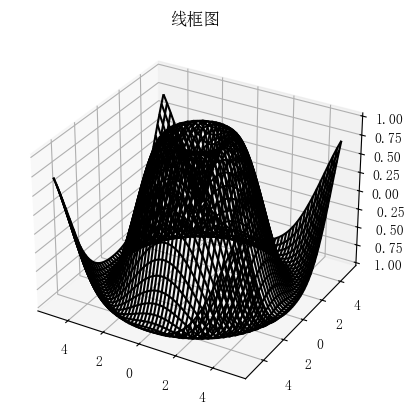
\includegraphics[width=0.6\textwidth]{part/图形化/Matplotlib/pic/绘图/线框图演示.png}
    \caption{线框图演示}
    \label{fig:线框图演示}
\end{figure}


\subsection{plt.plot\_surface 曲面图}
\codeinline{plt.plot\_surface()} 用于绘制曲面图。
\begin{lstlisting}[style=demostyle,numbers=none]
# 必须导入的库
import matplotlib.pyplot as plt
from mpl_toolkits.mplot3d import Axes3D
# plot_surface 功能：绘制曲面图
plt.plot_surface(X, Y, Z, cmap=None, **kwargs)
# 参数说明：
# X, Y, Z : 网格数据
# cmap : 颜色映射
\end{lstlisting}
\begin{lstlisting}[style=pythonstyle]
import matplotlib.pyplot as plt
import numpy as np
from mpl_toolkits.mplot3d import Axes3D

# 数据
x = np.linspace(-5, 5, 50)
y = np.linspace(-5, 5, 50)
X, Y = np.meshgrid(x, y)
Z = np.sin(np.sqrt(X**2 + Y**2))

# 绘制曲面图
fig = plt.figure()
ax = fig.add_subplot(111, projection='3d')
ax.plot_surface(X, Y, Z, cmap='viridis')
plt.title('曲面图')
plt.show()
\end{lstlisting}
\begin{figure}[htpb]
    \centering
    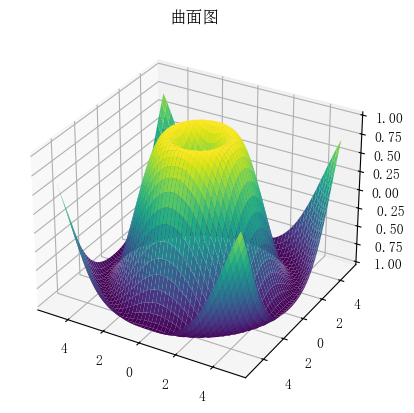
\includegraphics[width=0.6\textwidth]{part/图形化/Matplotlib/pic/绘图/曲面图演示.png}
    \caption{曲面图演示}
    \label{fig:曲面图演示}
\end{figure}

\begin{example}
    \exProblem
    绘制函数 $f(x, y) = (x^2 + y^2)\sin\left(\frac{1}{x^2 + y^2}\right)$ 的三维曲面图。

    \exSolution
\begin{lstlisting}[style=pythonstyle]    
import numpy as np
import matplotlib.pyplot as plt
from mpl_toolkits.mplot3d import Axes3D

# 定义函数 f(x, y)
def f(x, y):
    with np.errstate(divide='ignore', invalid='ignore'):
        z = (x**2 + y**2) * np.sin(1 / (x**2 + y**2))
        z[np.isnan(z)] = 0  # 处理 x^2 + y^2 = 0 的情况，避免除以零
        z[np.isinf(z)] = 0  # 处理无穷大的情况
    return z

# 创建 x 和 y 的网格数据
x = np.linspace(-1, 1, 300)
y = np.linspace(-1, 1, 300)
X, Y = np.meshgrid(x, y)

# 计算函数值
Z = f(X, Y)

# 创建三维图像
fig = plt.figure(figsize=(10, 8))
ax = fig.add_subplot(111, projection='3d')

# 绘制三维曲面图
surf = ax.plot_surface(X, Y, Z, cmap='viridis')

# 添加颜色条
fig.colorbar(surf, ax=ax, shrink=0.5, aspect=5)

# 设置标题和标签
ax.set_title(r'$f(x, y) = (x^2 + y^2)\sin\left(\frac{1}{x^2 + y^2}\right)$')
ax.set_xlabel('X axis')
ax.set_ylabel('Y axis')
ax.set_zlabel('Z axis')

# 显示图像
plt.show()
\end{lstlisting}

\begin{figure}[htpb]
    \centering
    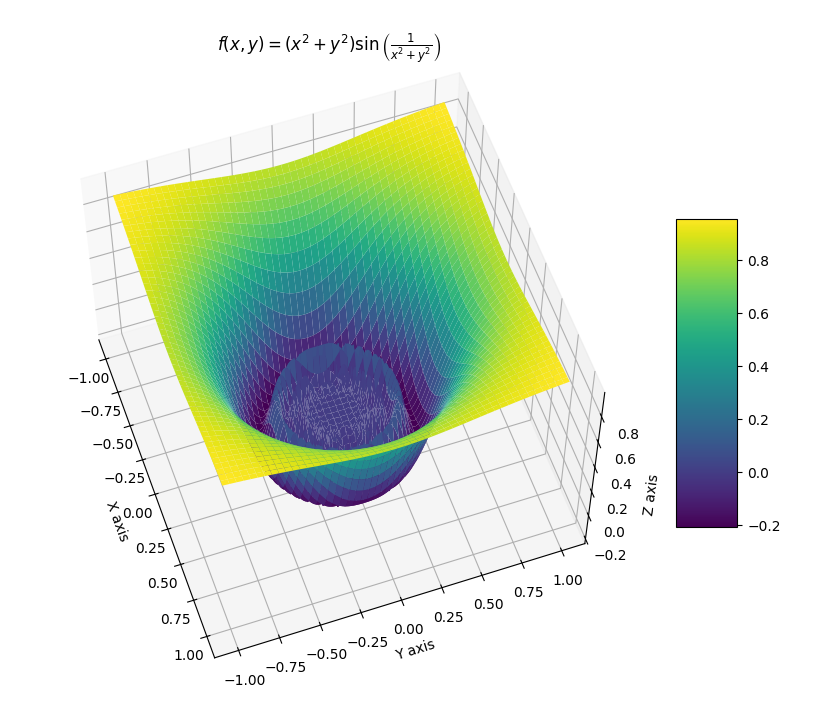
\includegraphics[width=0.6\textwidth]{part/图形化/Matplotlib/pic/绘图/曲面图surface_例题1.png}
    \caption{曲面图 $f(x, y) = (x^2 + y^2)\sin\left(\frac{1}{x^2 + y^2}\right)$}
    \label{fig:曲面图surface_例题1}
\end{figure}

\end{example}



\subsubsection{plt.plot\_surface 极坐标曲面图}
极坐标曲面图的绘制可以通过曲面的极坐标变换实现

\begin{lstlisting}[style=pythonstyle]
import matplotlib.pyplot as plt
import numpy as np
from mpl_toolkits.mplot3d import Axes3D

# 数据
r = np.linspace(0, 1, 50)
p = np.linspace(0, 2*np.pi, 50)
R, P = np.meshgrid(r, p)
Z = R**2

# 极坐标转化为笛卡尔坐标
X = R * np.cos(P)
Y = R * np.sin(P)

# 绘制极坐标曲面图
fig = plt.figure()
ax = fig.add_subplot(111, projection='3d')
ax.plot_surface(X, Y, Z, cmap='viridis')
plt.title('极坐标曲面图')
plt.show()
\end{lstlisting}

\subsubsection{plt.plot\_trisurf 曲面三角剖分}
\codeinline{plt.plot\_trisurf()} 用于绘制曲面三角剖分图。
\begin{lstlisting}[style=demostyle,numbers=none]
# 必须导入的库
import matplotlib.pyplot as plt
from mpl_toolkits.mplot3d import Axes3D
# plot_trisurf 功能：绘制曲面三角剖分
plt.plot_trisurf(x, y, z, cmap=None, **kwargs)
# 参数说明：
# x, y, z : 三维坐标
# cmap : 颜色映射
\end{lstlisting}
\begin{lstlisting}[style=pythonstyle]
import matplotlib.pyplot as plt
import numpy as np
from mpl_toolkits.mplot3d import Axes3D

# 数据
x = np.random.rand(100) * 10
y = np.random.rand(100) * 10
z = np.sin(np.sqrt(x**2 + y**2))

# 绘制曲面三角剖分图
fig = plt.figure()
ax = fig.add_subplot(111, projection='3d')
ax.plot_trisurf(x, y, z, cmap='viridis', edgecolor='none')
plt.title('曲面三角剖分')
plt.show()
\end{lstlisting}

